%% LyX 2.0.3 created this file.  For more info, see http://www.lyx.org/.
%% Do not edit unless you really know what you are doing.
\documentclass[english]{beamer}
\usepackage{mathptmx}
\usepackage[T1]{fontenc}
\usepackage[latin9]{inputenc}
\usepackage{color}
\usepackage{amsmath}
\usepackage{amssymb}

\makeatletter
%%%%%%%%%%%%%%%%%%%%%%%%%%%%%% Textclass specific LaTeX commands.
 % this default might be overridden by plain title style
 \newcommand\makebeamertitle{\frame{\maketitle}}%
 \AtBeginDocument{
   \let\origtableofcontents=\tableofcontents
   \def\tableofcontents{\@ifnextchar[{\origtableofcontents}{\gobbletableofcontents}}
   \def\gobbletableofcontents#1{\origtableofcontents}
 }
 \long\def\lyxframe#1{\@lyxframe#1\@lyxframestop}%
 \def\@lyxframe{\@ifnextchar<{\@@lyxframe}{\@@lyxframe<*>}}%
 \def\@@lyxframe<#1>{\@ifnextchar[{\@@@lyxframe<#1>}{\@@@lyxframe<#1>[]}}
 \def\@@@lyxframe<#1>[{\@ifnextchar<{\@@@@@lyxframe<#1>[}{\@@@@lyxframe<#1>[<*>][}}
 \def\@@@@@lyxframe<#1>[#2]{\@ifnextchar[{\@@@@lyxframe<#1>[#2]}{\@@@@lyxframe<#1>[#2][]}}
 \long\def\@@@@lyxframe<#1>[#2][#3]#4\@lyxframestop#5\lyxframeend{%
   \frame<#1>[#2][#3]{\frametitle{#4}#5}}
 \newenvironment{topcolumns}{\begin{columns}[t]}{\end{columns}}
 \def\lyxframeend{} % In case there is a superfluous frame end

%%%%%%%%%%%%%%%%%%%%%%%%%%%%%% User specified LaTeX commands.
\usetheme{Warsaw}
% or ...

\setbeamercovered{transparent}
% or whatever (possibly just delete it)

\makeatother

\usepackage{babel}
\begin{document}

\title{Sviluppi Teorici e Applicativi delle Metriche Entropiche di Rohlin}


\author{Dawid Crivelli }


\date{26 Aprile 2012}

\makebeamertitle

\lyxframeend{}\lyxframe{Sommario}

\tableofcontents{}


\lyxframeend{}\section{Distanze Entropiche}


\lyxframeend{}\lyxframe{Proteine dell'influenza H3N2}
\begin{topcolumns}%{}


\column{0.5\textwidth}
\begin{itemize}
\item sottotipi H1N1 e H3N2
\item sequenze lunghe 566 simboli
\item alfabeto di 24 lettere
\item solo 10\% mutazioni
\item \emph{antigenic drift}
\end{itemize}

\column{0.5\textwidth}
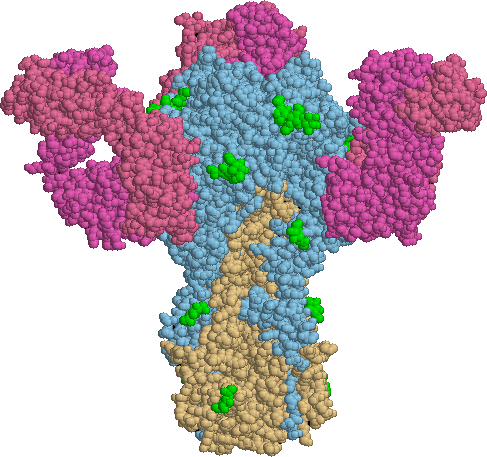
\includegraphics[0.5\textwidth]{../immagini/proteina_HA_3d}
\end{topcolumns}%{}
Sequenze
\lyxframeend{}\lyxframe{Hamming � poco adatto}


\lyxframeend{}\lyxframe{Distanza di Rohlin}


\lyxframeend{}\lyxframe{Applicabile su molte strutture}


\lyxframeend{}\lyxframe{Prodotti tra partizioni}


\lyxframeend{}\lyxframe{Partizionamento}


\lyxframeend{}\lyxframe{Intersezione tra partizioni}


\lyxframeend{}\lyxframe{Riduzione e amplificazione della distanza}


\lyxframeend{}\lyxframe{Definizione topologica della distanza}


\lyxframeend{}\lyxframe{Clustering di sequenze}


\lyxframeend{}\lyxframe{La riduzione lineare funziona meglio}


\lyxframeend{}\section{Sistemi magnetici}


\lyxframeend{}\lyxframe{Sequenze lineari di spin (Ising 1D)}


\lyxframeend{}\lyxframe{Clusters di spin $\Longleftrightarrow$ Clusters di link}


\lyxframeend{}\lyxframe{Lunghezza di correlazione tra partizioni}


\lyxframeend{}\lyxframe{Variazione in temperatura}


\lyxframeend{}\lyxframe{Tipi di disordine}


\lyxframeend{}\lyxframe{Ising 2D, reticolo quadrato}


\lyxframeend{}\section*{Summary}


\lyxframeend{}\lyxframe{Summary}
\begin{itemize}
\item The \textcolor{red}{first main message} of your talk in one or two
lines.
\item The \textcolor{red}{second main message} of your talk in one or two
lines.
\item Perhaps a \textcolor{red}{third message}, but not more than that.
\end{itemize}


\vskip0pt plus.5fill
\begin{itemize}
\item Outlook

\begin{itemize}
\item What we have not done yet.
\item Even more stuff.
\end{itemize}
\end{itemize}

\lyxframeend{}

\appendix

\lyxframeend{}\section*{Appendix}


\lyxframeend{}\subsection*{For Further Reading}


\lyxframeend{}\lyxframe{[allowframebreaks]For Further Reading}

\beamertemplatebookbibitems
\begin{thebibliography}{References}
\bibitem{Author1990}A. Author. \newblock\emph{Handbook of Everything}.\newblock
Some Press, 1990.\beamertemplatearticlebibitems

\bibitem{Someone2002}S. Someone.\newblock On this and that\emph{.}
\newblock\emph{Journal on This and That}. 2(1):50--100, 2000.

\end{thebibliography}

\lyxframeend{}
\end{document}
